% !TeX root = plotnikov_anton_cv.tex

\documentclass{cv}

\usepackage{datetime}
\usepackage[super]{nth}
\usepackage{fontawesome5}
\usepackage{tikz}
\usepackage[T2A]{fontenc}
\usepackage[russian]{babel}

\begin{document}

\cvheading{Плотников Даниил Михайлович}{%
	\begin{tikzpicture}
		\clip (0,0) circle (2cm);
		\node at (0,0) {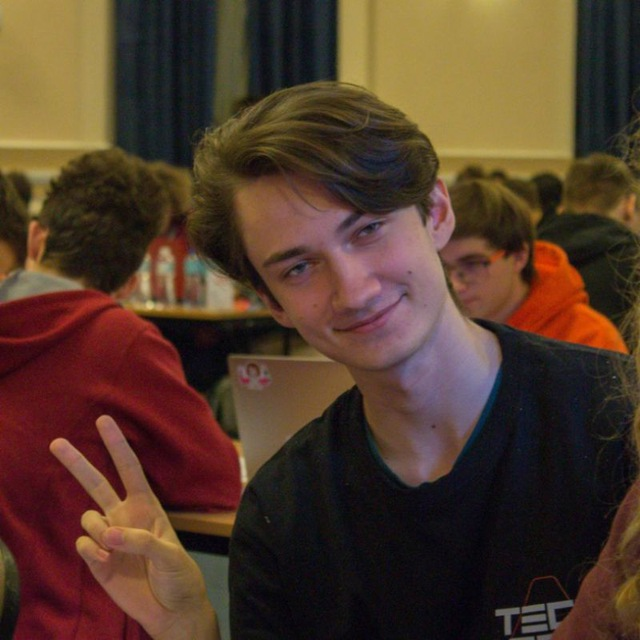
\includegraphics[width=4cm]{portrait.jpg}};
	\end{tikzpicture}%
}{%
	\begin{tabular}{cl}
		\faEnvelope      & \href{mailto:d.m.plotnikov04@gmail.com}{d.m.plotnikov04@gmail.com} \\
		\faTelegramPlane & \href{https://t.me/PlotDaniil}{@PlotDaniil}                          \\
		\faGithub*       & \href{https://github.com/Pepengu}{github.com/Pepengu}          \\
		\faMapPin        & Санкт-Петербург, Россия
	\end{tabular}%
}

\vspace{2em}


\section{Основные технологии}

\begin{cvblock}{I}
	Rust, C/C++, Linux, Docker, Git
\end{cvblock}

\begin{cvblock}{II}
	Nix (NixOS), \LaTeX, PostgreSQl
\end{cvblock}

\begin{cvblock}{III}
    Lua, Bash, Python
\end{cvblock}


\section{Опыт}


\begin{cvblock}{Open source}
	\begin{itemize}
		\item MARTOS
		      (\url{IvanArkhipov1999/Martos}):
              Martos — это элегантная операционная система реального времени, предназначенная для создания сложных мультиагентных систем. Разработчики имеют возможность писать программное обеспечение для Martos на языках Rust (предпочтительно) или C.
      \end{itemize}
\end{cvblock}

\begin{cvblock}{Преподаватель}
    \begin{itemize}
        \item Курс Спортивного Программирования СПбГУ 2024-н.в.
        \item Выездные школы СПбГУ «Электроника и программирование микроконтроллеров Arduino» 2024-н.в.
        \item Выездные школы СПбГУ «Спортивное программирование» 2024-н.в.
    \end{itemize}
\end{cvblock}

\begin{cvblock}{Организатор}
    \begin{itemize}
        \item I Чемпионат ПМ-ПУ 2024г
    \end{itemize}
\end{cvblock}

\section{Образование}

\begin{cvblock}{%
    \blocktitle
        {СПбГУ}
        {Санкт-Петербург}
        {}
        {2022--2026}
    }
    \textit{Факультет Прикладной Математики и Процессов Управления}
    \vspace{1em}

    \textit{Программирование и Информационные Технологии}
\end{cvblock}

\section{Языки}

\begin{cvblock}{Русский}
	Родной
\end{cvblock}

\begin{cvblock}{Английский}
	B2
\end{cvblock}

\vfill

\newdateformat{monthyear}{\monthname[\THEMONTH], \THEYEAR}
\begin{center}
	\monthyear\today
\end{center}

\end{document}
